% !TEX spellcheck = en_US


% In order to correctly compile this document,
% execute the following commands:
% 1. pdflatex
% 2. pdflatex
% 3. pdflatex



\documentclass[amsthm,ebook]{saparticle}

% IF YOU USE PDFLATEX
\usepackage[utf8x]{inputenc}
% if you write in english and in greek
\usepackage{ucs}
\usepackage[greek,english]{babel}
\languageattribute{greek}{polutoniko}

% IF YOU USE XELATEX
%\usepackage{polyglossia}
% if you write in italian
%\setmainlanguage{italian}
% If you want put some ancient greek:
%\setotherlanguage[variant=polytonic]{greek}
%\newfontfamily{\greekfont}[Ligatures=TeX]{Palatino Linotype}

% dummy text (remove in a normal thesis)
% remove if not necessary
\usepackage{siunitx}
%Natbib for bibliography management
\usepackage[authoryear]{natbib}
% custom commands
\newcommand{\bs}{\textbackslash}

%%%%%%%%
%TITLE:%
%%%%%%%%\title{}
\title{Working with Text and Images: The Graffiti of Herculaneum}
\author[WL]{Rebecca Benefiel\corref{first}}
\author[Millisaps]{Holly Sypniewski}
\author[WL]{Sara Sprenkle}\date{2015-11-19}
\address[WL]{Washington \& Lee University, United States of America}
\address[Millisaps]{Millsaps College, United States of America	}
\cortext[first]{Corresponding author. Email: benefielr@wlu.edu}	
\begin{document}

\maketitle
\begin{abstract}
We discuss several challenges encountered by our team as we digitize ancient graffiti, handwritten inscriptions scratched into wall-plaster, for the Epigraphic Database Roma and the Ancient Graffiti Project. Here, we focus on decisions we made in editing and digitizing not only textual graffiti but also the figural examples (hand-sketched drawings) that sometimes appear alongside them. We also discuss search capabilities that will allow users both to browse and search for figural graffiti.
\end{abstract}
\keywords{Ancient graffiti, figural images, contextualization, standards, Herculaneum}

\section{Introduction}

\noindent Our project is working with informal, handwritten wall-inscriptions, or ancient graffiti, which were scratched into the
wall-plaster of ancient towns. \ Several hundred of these handwritten inscriptions have been documented at Herculaneum
and more than 6000 are known from Pompeii. We are contributing these inscriptions to the Epigraphic Database Roma
(\url{www.edr-edr.it}), and are creating a linked resource, the Ancient Graffiti Project (\url{ancientgraffiti.wlu.edu}), that will
allow users to conduct location-specific searches for graffiti. 

Among the many texts written on the walls of these two cities, there sometimes also appear graffiti drawings, or figural
graffiti [Fig.~\ref{fig:1}]. 

\begin{figure}[!bp]
\centering
 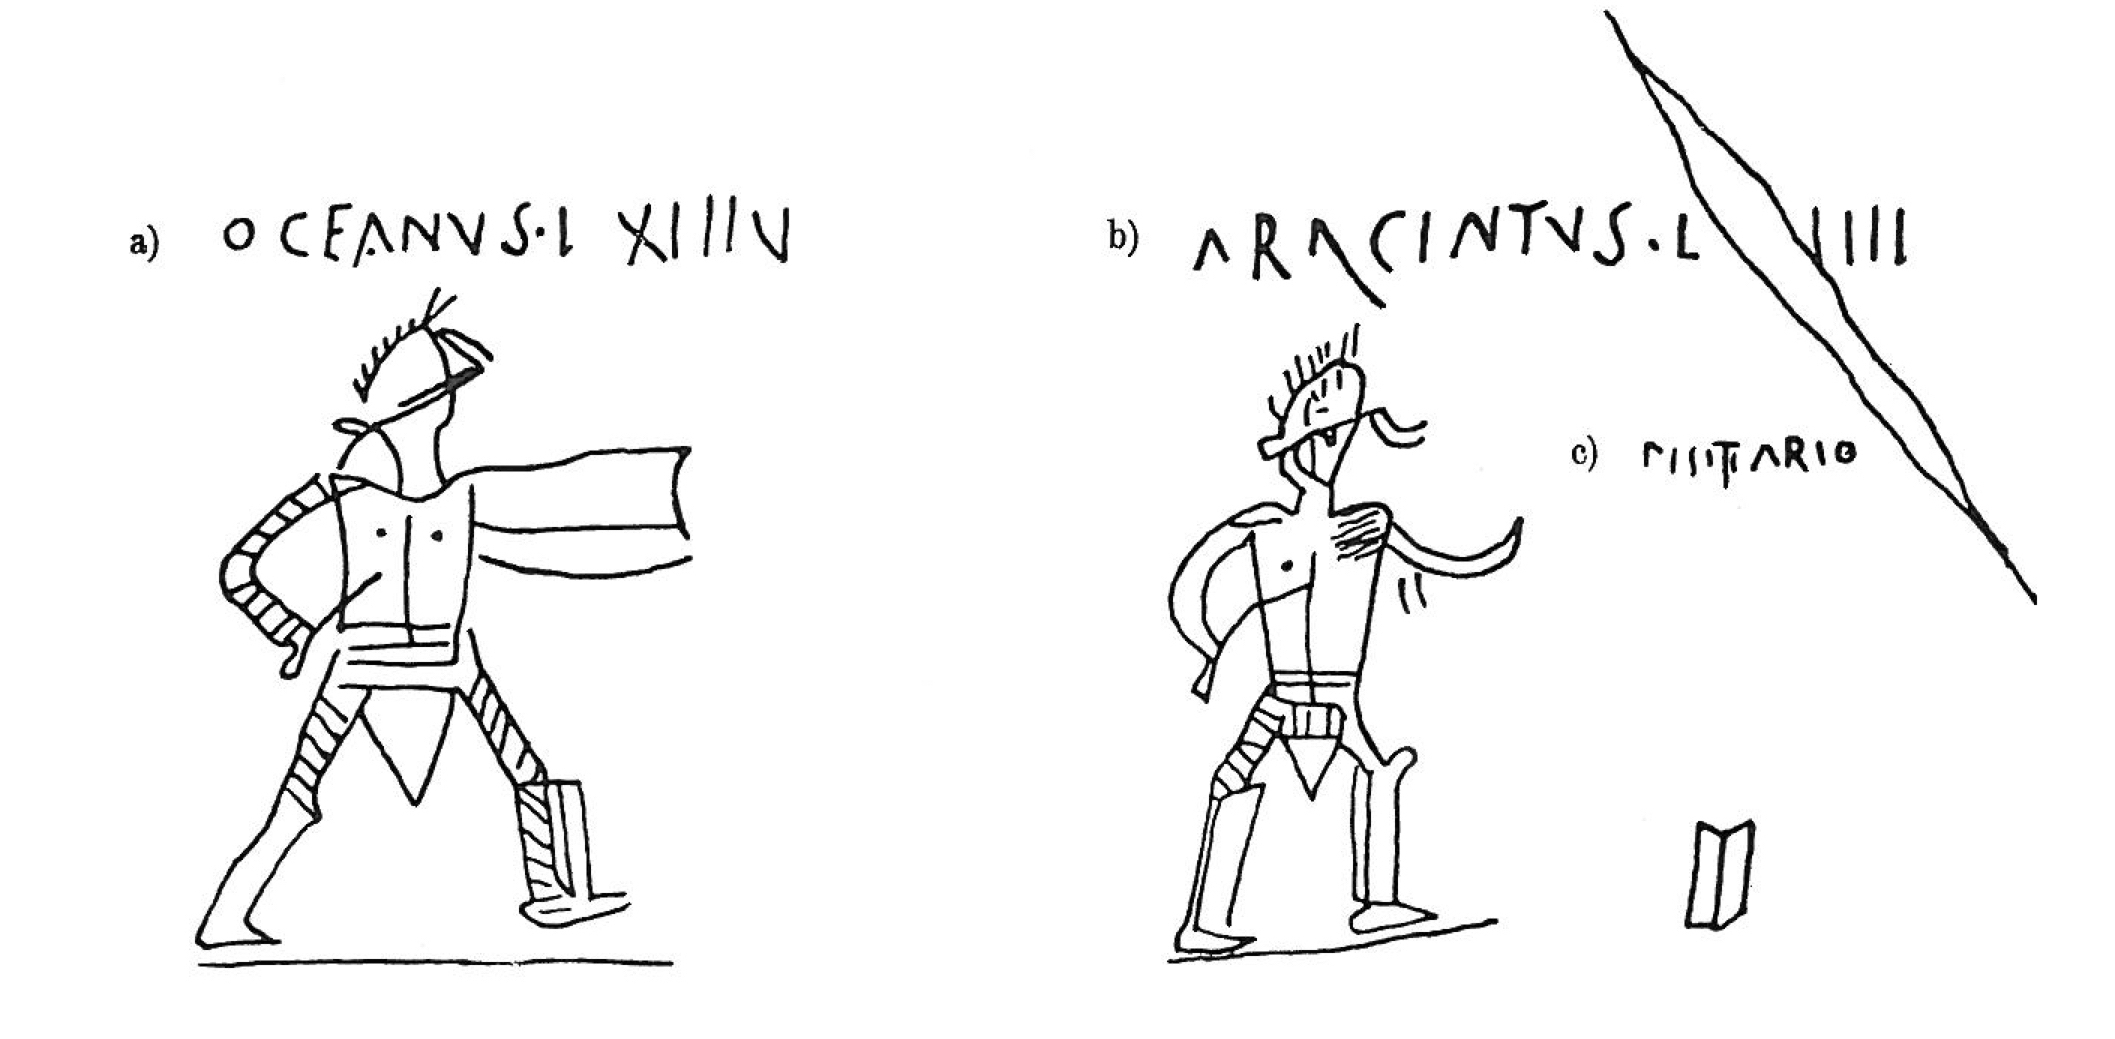
\includegraphics[width=\columnwidth]{EAGLE2016BenefielSypniewski-img001.jpg}
\caption{ Graffito from Pompeii [\emph{CIL} 4, 5215]}
\label{fig:1}
\end{figure}


This graffito depicts a pair of gladiators, where the two figures are identified with their names and the number of
their victories. The inscription therefore includes both text and image. It was much more common in Pompeii for someone
to write a message on a wall than to sketch a drawing: people wrote their names, greetings to friends, quotations of
literature, and other types of messages. However, we do find a smaller, but not insignificant number of drawings also
inscribed on the wall plaster throughout the town. It is very rare to find a large scene, like the illustration of a
gladiatorial contest with athletes, musicians, and perhaps magistrates, sketched by hand on a funerary monument just
outside the Porta Nocera of Pompeii (\emph{CIL} 4, 10237; \citet[D31]{cooley_pompeii_2013}; cf. also \emph{CIL} 4, 10236 and 10238 drawn
nearby). \ More commonly, people made small sketches on the walls around them choosing from roughly a handful of
popular designs: \ heads in profile, boats, gladiators, birds, and geometric designs \citep{langner_antike_2001}.




Figural graffiti have provided us with several challenges as we digitize them for the Epigraphic Database Roma and as we
design a way to search for and retrieve such drawings via the Ancient Graffiti Project search engine. In this paper we
will discuss the challenges we face and some of the strategies we have developed in response. 




\section{Our Material}
 

\noindent First, a little background on figural graffiti and our sources for this data. In Herculaneum, we are fortunate that a
significant number of graffiti are still extant and \emph{in situ}, as roofing has been reconstructed for many buildings to
protect them from the elements. Due to the fragile nature of wall plaster, however, especially in Pompeii, many
graffiti that were recorded previously and published in \emph{CIL} 4, have now been lost. Much of our data, therefore, comes
from verbal descriptions of graffiti that have since disappeared. Furthermore, the different editors of \emph{CIL} 4 and its
supplements used different methods to denote that a drawing was present, and their practices changed over time. Working
with this legacy data, therefore, presents a range of difficulties. 




\subsection{Verbal Descriptions of Figural Graffiti Found With Text}

\begin{figure}[!bp]
\centering
 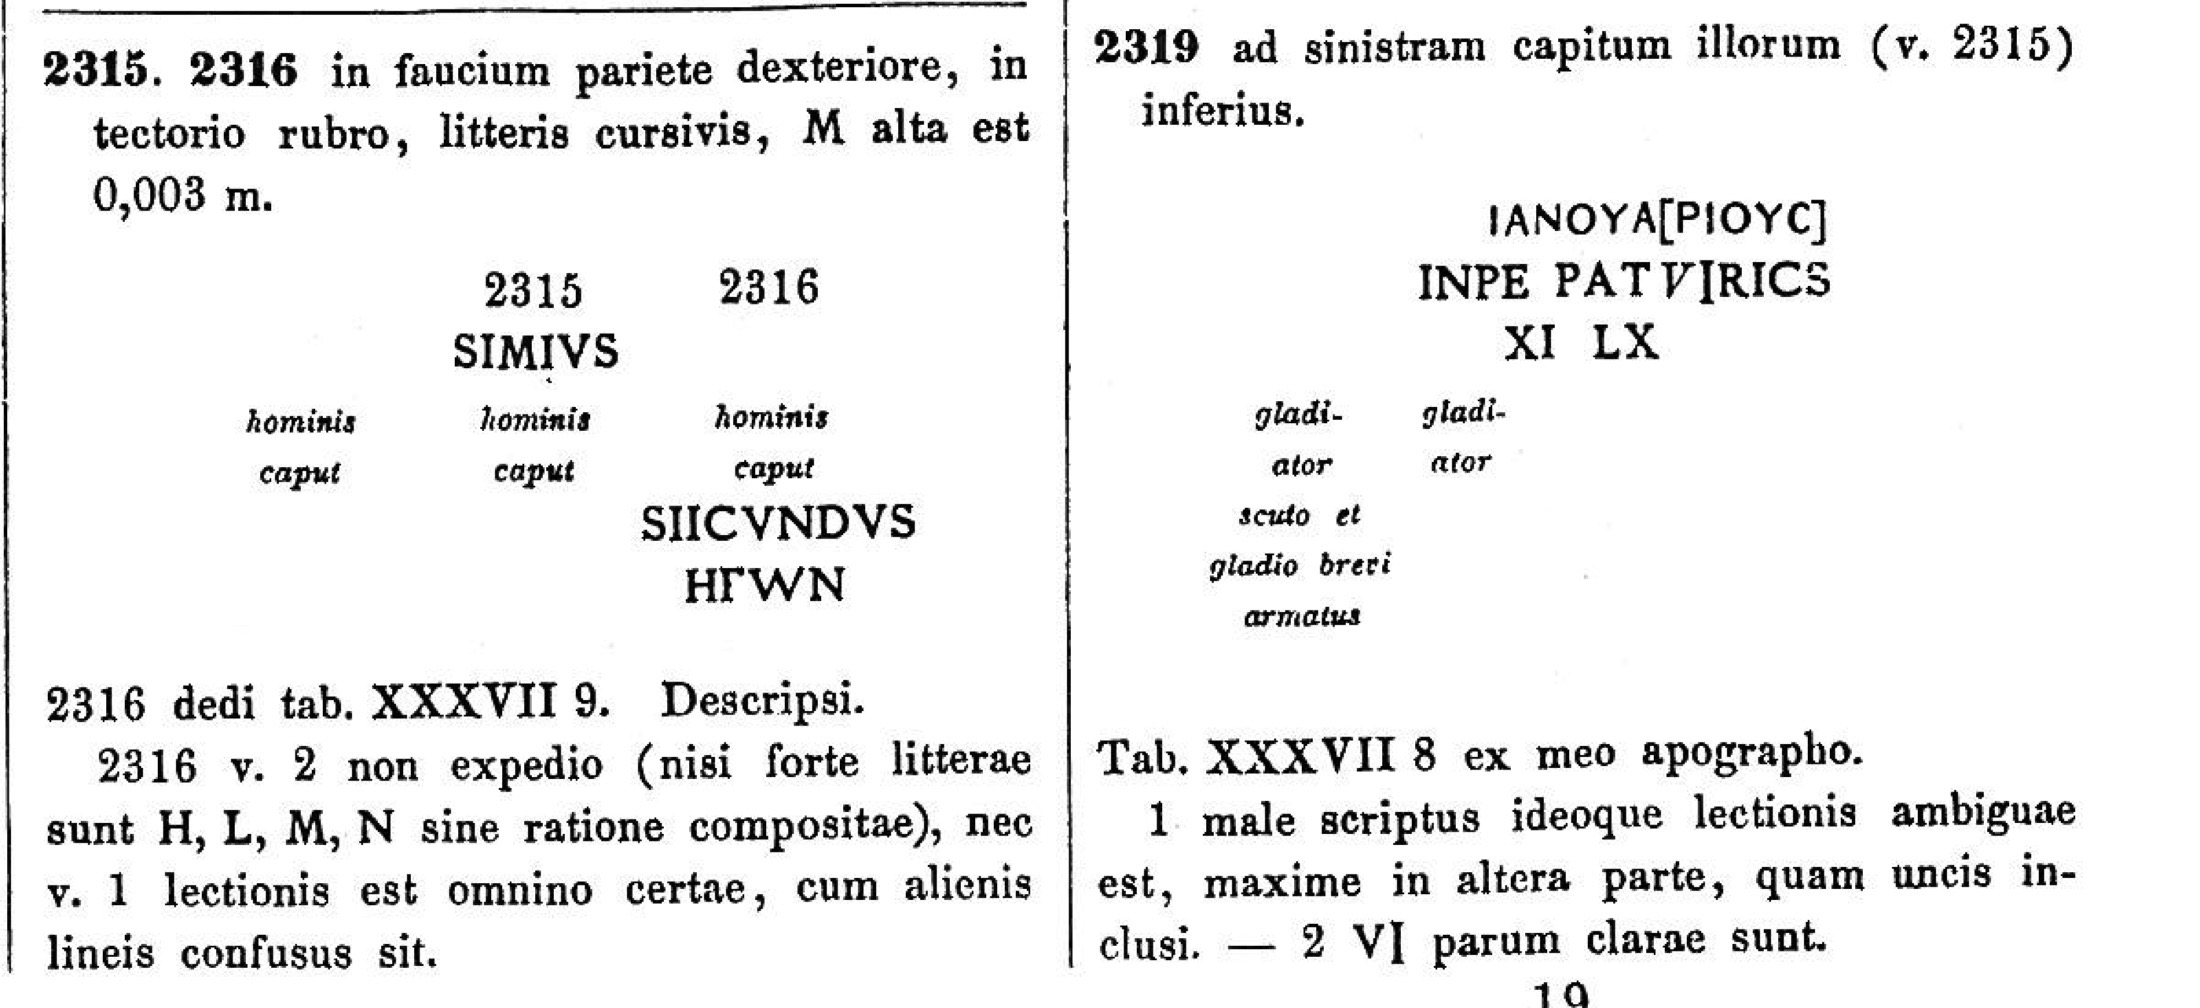
\includegraphics[scale=0.15]{EAGLE2016BenefielSypniewski-img002.jpg}
\caption{The entries of \emph{CIL} 4, 2315-2316 and 2319, representing figural graffiti via brief description}
\label{fig:2}
\end{figure}


A drawing could, for example, be described in the text field of an entry in \emph{CIL} 4. This occurs in the entries below,
where three drawings of human heads [\emph{CIL} 4, 2315-2316] and two drawings of gladiators [\emph{CIL} 4, 2319] are described in
small italics, placed where the images occur alongside the textual inscriptions [Fig.~\ref{fig:2}]. 



The italics make clear that those descriptions are not part of the texts of the inscriptions themselves, which are
represented in capital letters.




This practice is common in the original volume of \emph{CIL} 4, when it seems that the editors documented textual and
figural graffiti that were in close proximity, or that were in some way related to each other. In later supplements,
line-drawings for figural graffiti were sometimes included when the drawings and text were obviously understood as one
inscription, as shown in Fig. 1 above. Perhaps due to the complications with preparing and printing such
illustrations, however, it also remained common practice to represent figural graffiti with very brief description in
italics (e.g. \emph{CIL} 4, 4822, 4823, 5264, 5275, 6624, 6672, 6889). 




\subsection{Figural Graffiti described in notes or apparatus}


\noindent The most common strategy, however, for documenting figural graffiti in \emph{CIL} 4 is by including brief mention of a drawing
in the editorial note that introduces a graffito or in the apparatus that follows it [Fig.~\ref{fig:3}].  



\begin{figure}[!bp]
\centering
 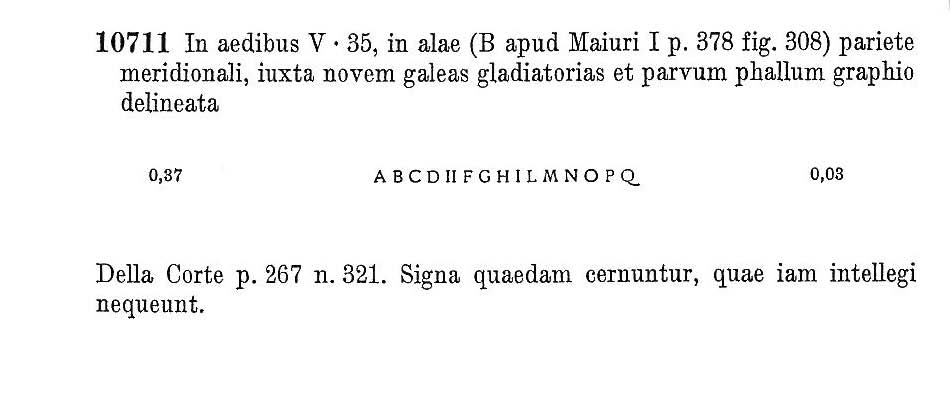
\includegraphics[width=\columnwidth]{EAGLE2016BenefielSypniewski-img003.jpg}
\caption{\emph{CIL} entry for an alphabet near figural graffiti [\emph{CIL} 4, 10711]}
\label{fig:3}
\end{figure}
 


Note that the editorial note above the entry mentions drawings nearby (\emph{novem galeas gladiatorias et parvum phallum}), but
the text is presented without illustration. This mode becomes more common in the fascicles of \emph{CIL} 4 produced in the
later twentieth century and so the figural graffiti from Herculaneum are usually represented this way (cf. \emph{CIL} 4,
10532, 10568, 10586). 




\subsection{Figural graffiti omitted by \emph{CIL}}


A fourth possibility exists as well, namely, when figural graffiti were not even mentioned in \emph{CIL}. In each of the
previous scenarios, the editors of \emph{CIL} include a description of a figural graffito when it was close to a textual
inscription. In contrast, figural graffiti found in isolation tended to be excluded altogether due to the focus of the
\emph{Corpus} on text. Fortunately there is now a useful resource devoted to figural graffiti: Martin Langner’s \emph{Antike
Graffitizeichnungen}, a monograph and accompanying database of figural graffiti from across the Mediterranean. His
catalog includes some 600 graffiti drawings from Pompeii and 60 from Herculaneum, including 200 that are not mentioned
in \emph{CIL}. In addition, whenever possible, Langner will provide a line-drawing of the graffito, either his own or one
found in an earlier source; therefore, his database includes many line drawings that are not included in \emph{CIL} even when
a drawing is described. However, certain motifs are omitted from Langner’s catalog. While he does catalog the more
interesting \emph{Phalluskopfen} examples, he generally omits simple drawings of \emph{phalli}. He also leaves aside the decorative
elements of \emph{coronae} and \emph{palmae}, which are sometimes mentioned in \emph{CIL}. This means that an accurate total of all figural
graffiti in Pompeii and Herculaneum can only be reached by working through the collections of both Langner and \emph{CIL}. To
create the most comprehensive resource possible for figural graffiti, we include all known drawings in the AGP search
engine. 




\subsection{Documenting extant figural graffiti}


\noindent Since the verbal descriptions of figural graffiti provided by legacy data are limited and vague or exceedingly general
(e.g. \emph{caput}), the best circumstance under which to digitize a graffito is when the drawing itself still remains extant.
 In such cases, we will use any published data as a starting point, but we are also able to make our own editorial
decisions about the subject matter of the drawing, how to describe it, and its relation to any text that is nearby.
The material with which we are working, therefore, includes a range of different information about the figural
graffiti of Pompeii and Herculaneum: from brief verbal descriptions to line-drawings, to the best case scenario when an
inscription is still extant. 

\section{Challenges in working with text and images}


Several challenges, therefore, arise when making decisions about how to edit and digitize figural graffiti. These can
depend on how a drawing may or may not relate to a textual graffito, whether or not a drawing is extant, and how to
interpret and standardize legacy data. 




Three of our main questions are:

\begin{enumerate}
\item \textbf{How to define an entry?} (Where for example does one entry stop and another begin? Do we catalog series or clusters
of graffiti, or individual images? How do we account for or represent the larger context?)
\item \textbf{How to describe a drawing?} (Here, there arise issues both of standardization and of interpretation, or over
interpretation.)
\item \textbf{How can we make drawings searchable?} (Ideally, we would like to make it possible for users both to browse and to
locate specific images.)
\end{enumerate}



\subsection{How to define an epigraphic entry?}
 

One of the first challenges we face in working with figural graffiti is deciding how to define an entry, that is, to
consider whether or not multiple elements should be part of the same EDR record or should be given separate entries.
First, we must ask: \emph{can we be assured} that certain elements were meant to be understood together? There might be an
issue of accretion or accumulation, where additional graffiti have been added subsequently. A related challenge is
then, if we create individual entries for separate elements, how do we avoid losing information about the relationship
among the graffiti? This collection of drawings including six textual graffiti illustrates our challenge [Fig.~\ref{fig:4}].

\begin{figure}[!bp]
\centering
 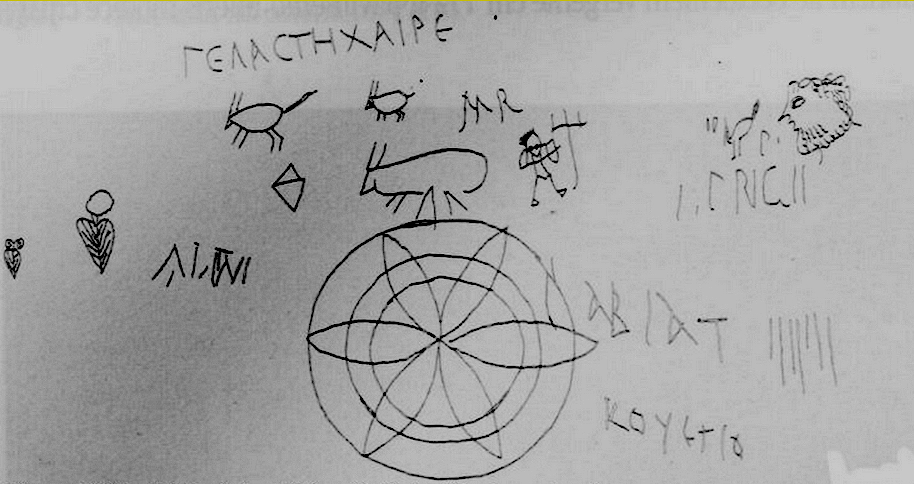
\includegraphics[width=\columnwidth]{EAGLE2016BenefielSypniewski-img004.jpg}
\caption{Line-drawing displaying a collection of textual and figural graffiti [\emph{CIL} 4, 8383-8386; EDR148730]; unpublished
sketch of Matteo Della Corte from the archives of the \emph{Corpus Inscriptionum Latinarum} at the Berlin-Brandenburg Academy
of Science and Humanities.}
\label{fig:4}
\end{figure}




You can see a number of different images here including a small gladiator with trident, a face in profile, leaves,
several animals, and geometric shapes as well as the name ``Atini'' and the greeting ``\textgreek{Γελαστὴ χαῖρε}.'' Such a collection raises many interpretive questions. What is the relationship, if any, between the figural and the
textual graffiti? How should that relationship be best represented? Fortunately, we have available with this sketch an
overall view of the spatial relationships of this group of graffiti. Because the \emph{CIL} entries are focused on text, the
figural graffiti are associated with and described in the entry of nearby textual inscriptions. For this cluster, we
have decided, instead, to give each element on the wall a unique identifier. First, it is not clear that the texts are
clearly linked to any of the drawings. \ Secondly, if we create individual entries, the field for measurements in EDR
permits us to give the measurements for each individual element. Thirdly, EDR has provided an additional solution to
the issue of representing context with the use of hyperlinks to other nearby inscriptions, created by including EDR
record numbers in the apparatus field. Additionally, we have decided to upload a series of images to EDR, including
detail illustrations and the composite sketch of all graffiti, to give the context of the entire cluster and the
relationship of the graffiti to each other.

In an example from Herculaneum (Fig.~\ref{fig:3}, above), the entry for \emph{CIL} 4, 10711 notes that in addition to a graffito of the
alphabet, a series of nine gladiator helmets and a small phallus were also drawn on the wall. During our field season
in Herculaneum in 2014, we were not successful in finding the graffiti of the alphabet or small phallus, but we did
locate eight of the nine helmets. Here too we have devoted a separate database entry for each helmet. By making
individual records, we have a unique identifier for each image, in the form of the EDR number, so that users can cite a
\emph{specific} parallel precisely. \ Again, we can record the precise measurements for each image. Yet, since separating
each image can obscure how the images relate to one another in the group, as with the previous example, we also upload
to EDR an overall image of the group of helmets together for every individual entry (cf. EDR143634).

In these two cases, we are fortunate to have contextual data that informs our understanding of how text and image may
relate. More often, we are left with only legacy data, with brief mention of a figural graffito in the apparatus of a
\emph{CIL} entry and without illustration. \ Yet, proximity does not always indicate a relationship between the text and
image. \ Indeed, there may be no relationship at all between the figural and textual graffiti; therefore, putting the
two graffiti in the same EDR record may suggest a relationship where none exists. Given these circumstances, we prefer
to create separate EDR entries for the text and the image and to use the EDR hyperlinks to note that each is found near
the other.




\subsubsection{How to describe drawings? }


A second challenge occurs when we must decide how much interpretation to offer when we describe a graffito for a
database entry. \ When \emph{CIL} has included mention of a drawing, we generally incorporate that description directly into
our entry. With figural graffiti documented by Martin Langner, we must create a summary in Latin and when doing so, we
attempt to give as full as possible a description of the elements of the image. With this camel \citep[n. 1443]{langner_antike_2001}, for instance, we offer a full description in Latin that accounts for all the features of the drawing: \emph{camelus dromedarius cum cauda, lodicem gerens, ad dextram incedens} [Fig.~\ref{fig:5}].



\begin{figure}[!hbp]
\centering
 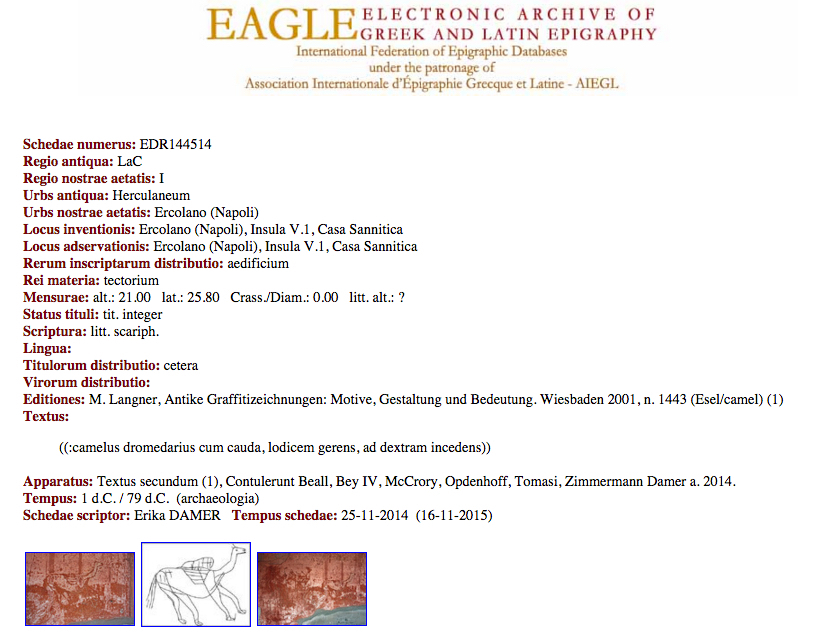
\includegraphics[width=\columnwidth]{EAGLE2016BenefielSypniewski-img005.jpg}
\caption{Example of an entry for a figural graffito not found in \emph{CIL} (EDR144514)}
\label{fig:5}
\end{figure}



\subsubsection{Questions of interpretation through description}


As one might imagine, issues of interpretation can arise even with simple descriptions of images. In truth, we have
encountered more difficulties with interpretation in the case of drawings that have been described by \emph{CIL}. The first
example comes from a shop in Pompeii and represents text and a drawing [\emph{CIL} 4, 8185]. \ The plaster has clearly broken
off, so we do not know if this was part of a larger scene. What remains are two lines of text and just one figure,
which would seem to be a drawing of a person facing forward and rendered with head and shoulders. \emph{CIL} describes it
thus: \emph{herma \underline{muliebris} prospiciens} [Fig.~\ref{fig:6}].
\newpage

\begin{figure}[!hbp]
\centering
 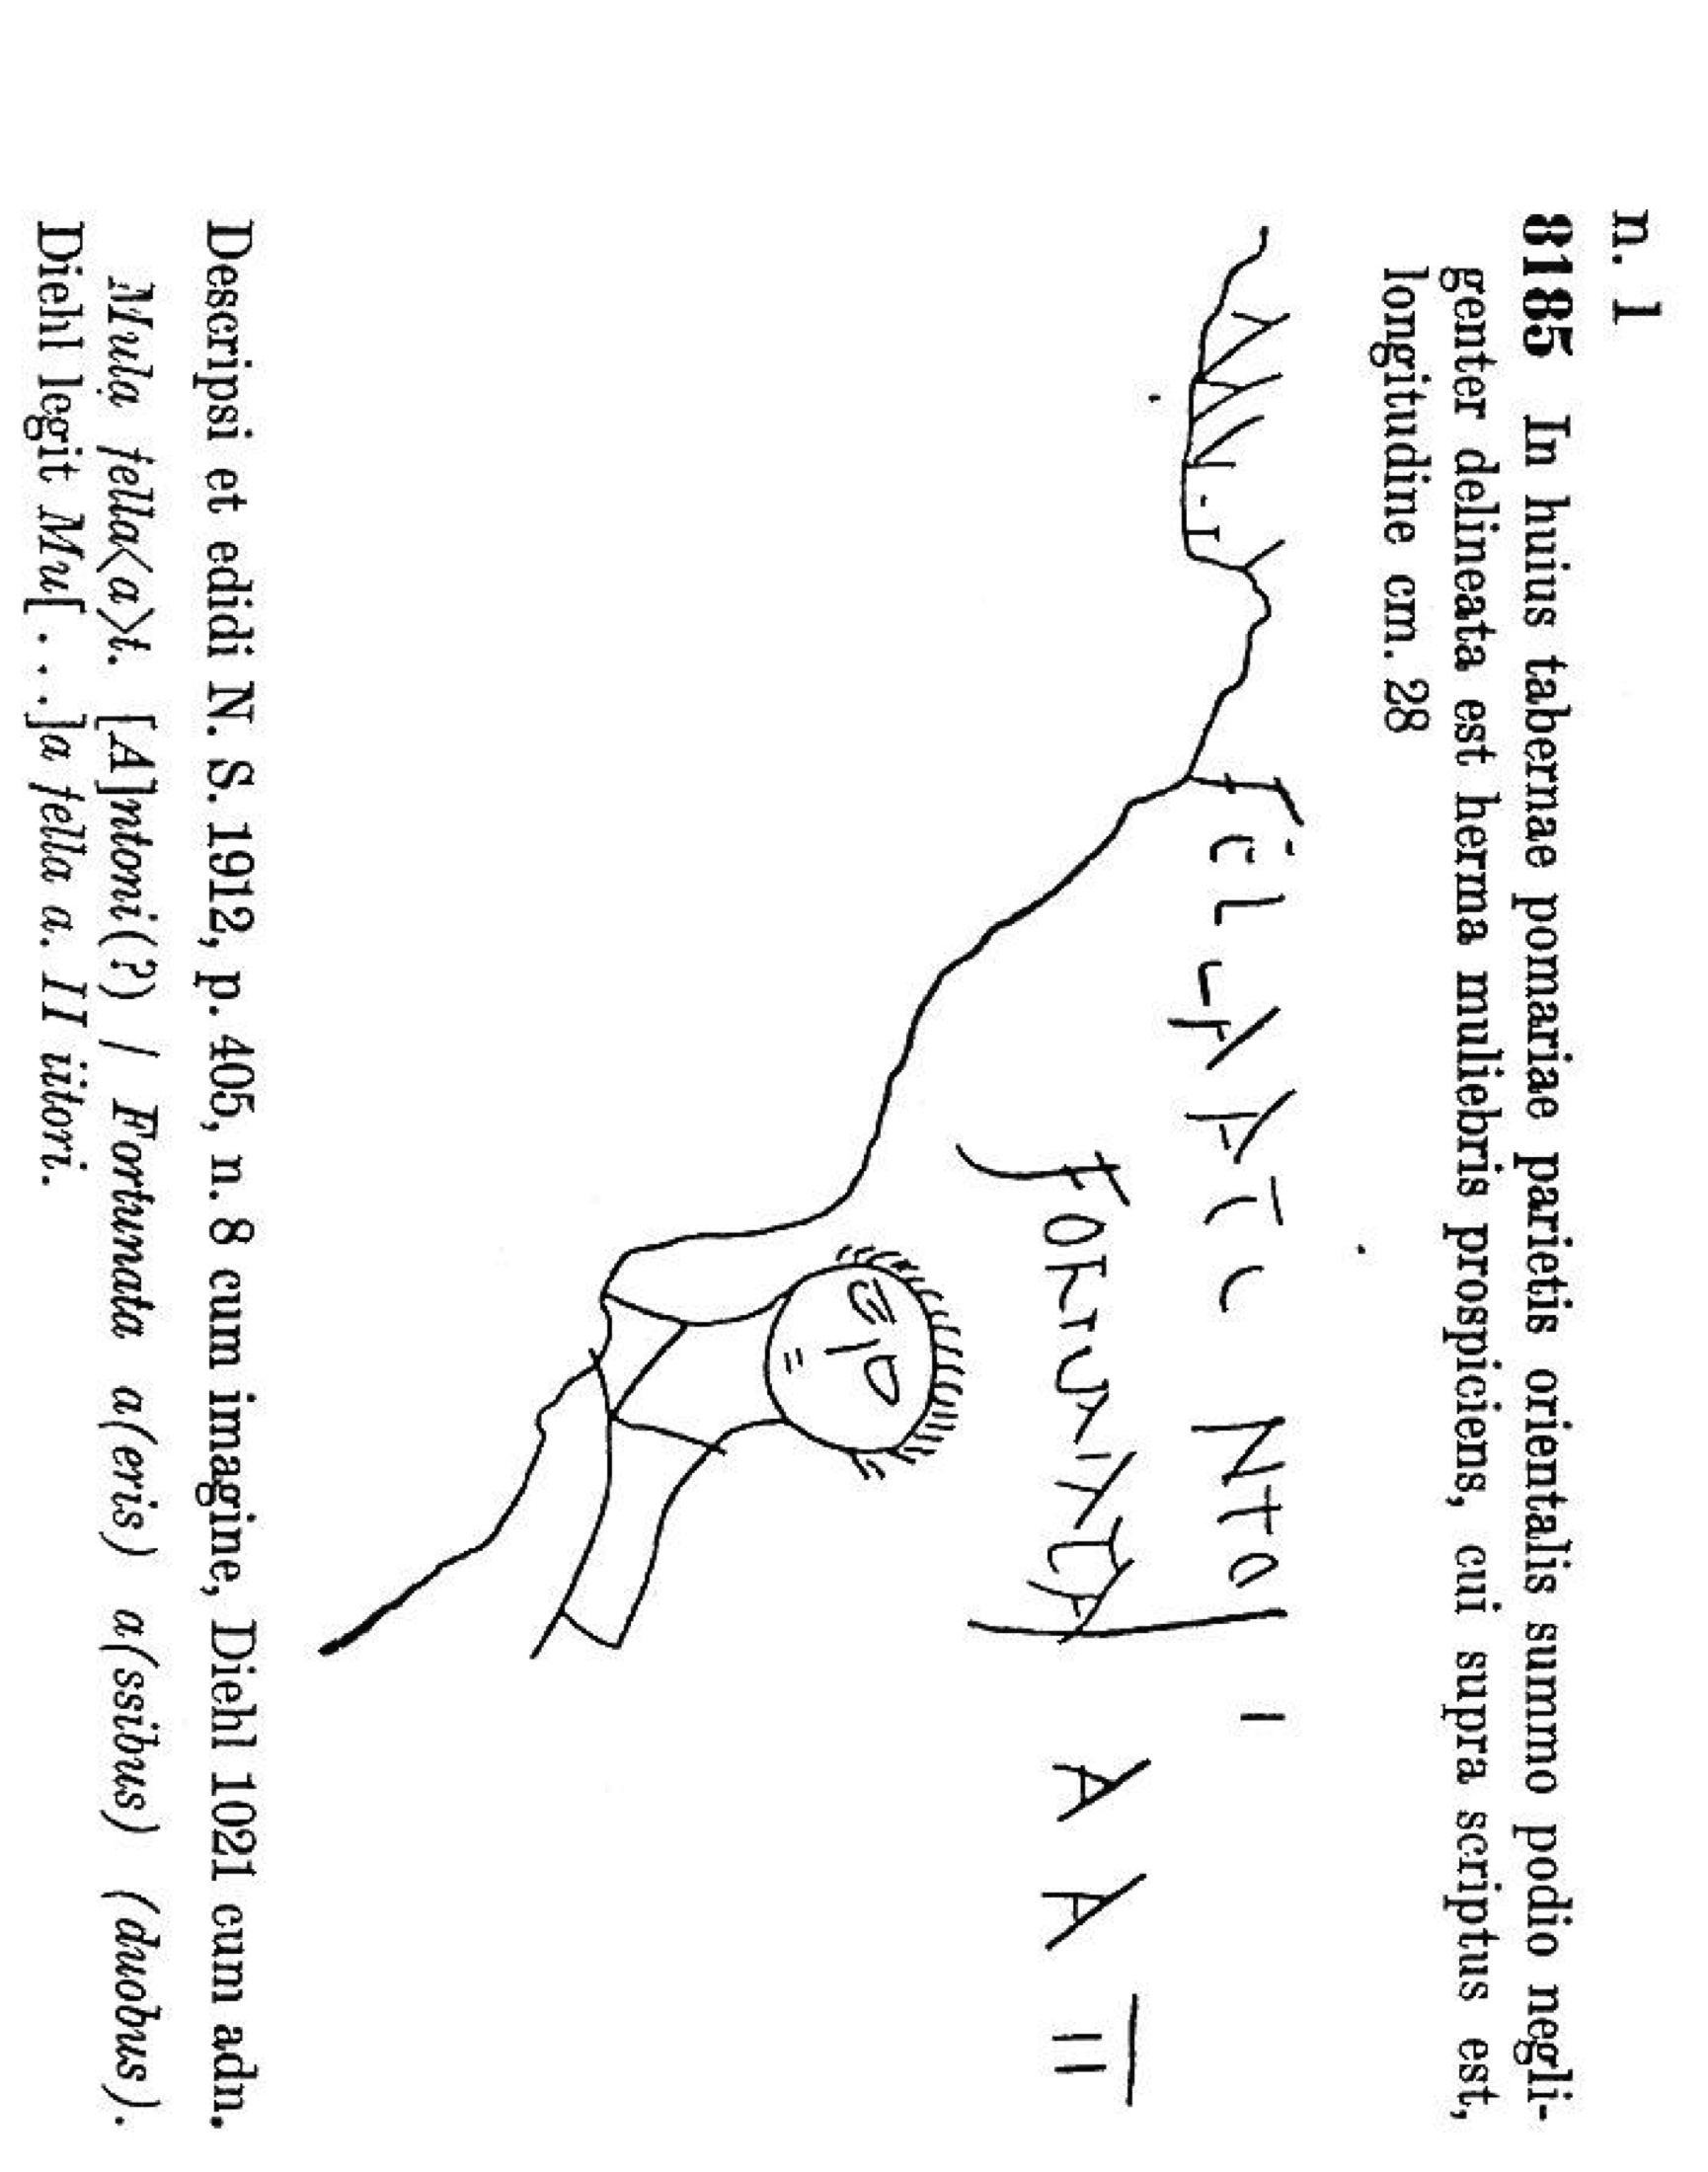
\includegraphics[width=\columnwidth]{EAGLE2016BenefielSypniewski-img006.jpg}
\caption{\emph{CIL} entry for textual and figural graffiti [\emph{CIL} 4, 8185]}
\label{fig:6}
\end{figure}




Is this drawing clearly depicting a female? It is difficult to argue from either the hairstyle or the clothing that the
figure is female. Here, we can only assume that the editors of \emph{CIL} identified the image as female because the text
above mentions the female name Fortunata. But are we sure the image is meant to illustrate the text? Or that the image
and text are meant to be read together? Since the figure is clearly not enacting the verb of the text, could this be
either Fortunata or Antonius?

The head of a woman, described with a textual graffito from the Suburban Baths in Herculaneum [\emph{CIL} 4, 10676], raises
similar problems with verbal descriptions of figural graffiti. In this case, \emph{CIL} does not reproduce an image of the
sketch; it only notes that the four-line inscription of \emph{CIL} 4, 10676 appears below a drawing of a female (\emph{infra
mulieris imaginem}). In this instance, too, the text nearby includes two names, one female and one male. The drawing has
appeared in multiple publications \citep{della_corte_loves_1960,deiss_herculaneum_1989,vivolo_pompei:_1993} [Fig.~\ref{fig:7}]. 



Again, we might question whether this figure should be identified as female. In fact, we not certain that we had located
the correct apograph for the drawing. There is considerable discrepancy between the description of the drawing in \emph{CIL}
4, 10676 as female, with no mention of the long nose, and this line-drawing. 


\begin{figure}[!hbp]
\centering
 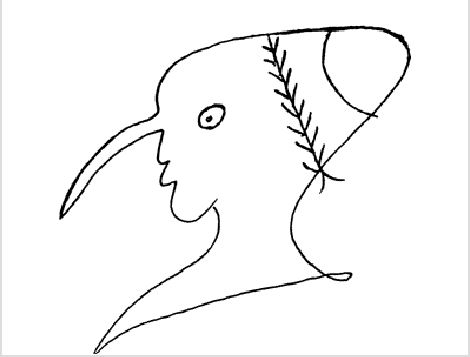
\includegraphics[width=\columnwidth]{EAGLE2016BenefielSypniewski-img007.jpg}
\caption{Apograph of figural graffito referred to in the note at \emph{CIL} 4, 10676 \citet[n. 309]{langner_antike_2001}.}
\label{fig:7}
\end{figure}


Another reason we suspected there might be a mistake was that Martin Langner had catalogued the drawing associated with
\emph{CIL} 4, 10676, describing it as a ``Phalluskopf.'' There was no mention of gender. And he categorized this drawing among
several examples of drawings of heads with phallic features. The graffito is in a room that is sealed off, with no
access, so we were unable to view it in person. Eventually, however, a photograph published by Antonio Varone in his
recent two-volume work providing images of extant ancient graffiti \citep[509]{varone_titulorum_2012} allowed us to confirm that this
is indeed the correct graffito drawing – somewhat above but also drawn partly \emph{through} the text of \emph{CIL} 4, 10676. 

Neither description offered by \emph{CIL} or by Langner, however, seems altogether satisfactory. There are no obvious markers
of female identity and even the description of \emph{Phalluskopf} is less than transparent. Thus this one drawing has two
published descriptions that vary greatly and that each lead to a very different understanding of the graffito. What
should we then do in such situations? Do we repeat the identification of \emph{CIL}? Or do we offer a less specific
description, merely labeling this a \emph{hominis figura}? In the end, our solution is to offer our own description, which
is detailed but less interpretative, with an emphasis on specific features of the image that are readily identifiable.
We also document Langner’s description and \emph{CIL}’s earlier identification in our entry for EDR, but we note our
hesitation with such identification by labeling the image: \emph{gryllus}? (``caricature?''). We are aware, however, that we
also introduce an interpretation with the tentative suggestion this drawing might be a caricature. 

The issue of interpretation arises most often in relation to identification. Other examples concern identifying the
particular types of gladiators or the species of animals, who are assuredly quadrupeds but in some drawings could be
any type of animal with four legs (stags, boars, dogs). In such cases, our solution is to describe a drawing with more
generic, yet accurate, terms such as ``gladiator,'' without further specification, or ``animal'' rather than \emph{cervus}, \emph{aper},
or \emph{canis}. Similarly, if we cannot determine male or female, we prefer to describe the drawing as ``\emph{facies hominis}.'' In
the AGP search engine we can then indicate possible but not certain identification with a descriptor, or tag, that
comes with a question mark: e.g. ``stag?'' 




\section{How to search for drawings?}


\noindent The third challenge that we face is how to search efficiently for inscriptions that are not just text but either are
images or include images. In the AGP search engine, we aim to complement the capabilities of EDR by providing another
way to search for these non-textual, figural graffiti. Since we describe the content of the figural graffito in the
Textus field of EDR, it is possible for a user to locate a graffito drawing. However, with text-based searching, a user
would need to need to know the vocabulary used to describe the drawing. Would someone ever think to search for
``\emph{camelus}'' without prior knowledge that there is a figural graffito of a camel in Herculaneum? Similarly, if you
search for ``\emph{gladiator}'', the text field will give you results for all inscriptions that mention gladiators as well as
drawings where we have described gladiators. If, however, we’ve described the gladiator more specifically as a
``\emph{retiarius}'' or we have gladiatorial equipment, such drawings will be omitted from the list of search results.
\newpage
We are therefore designing AGP with the capacity for locating figural graffiti through a two-prong solution: with
both browsing and searching possibilities. 




\subsection{Browsing capabilities in AGP}


\noindent For browsing, we have defined nine broad general categories, which together cover all the types of figural graffiti
we have encountered so far [Fig.~\ref{fig:8}]. 

\begin{figure}[!hbp]
\centering
 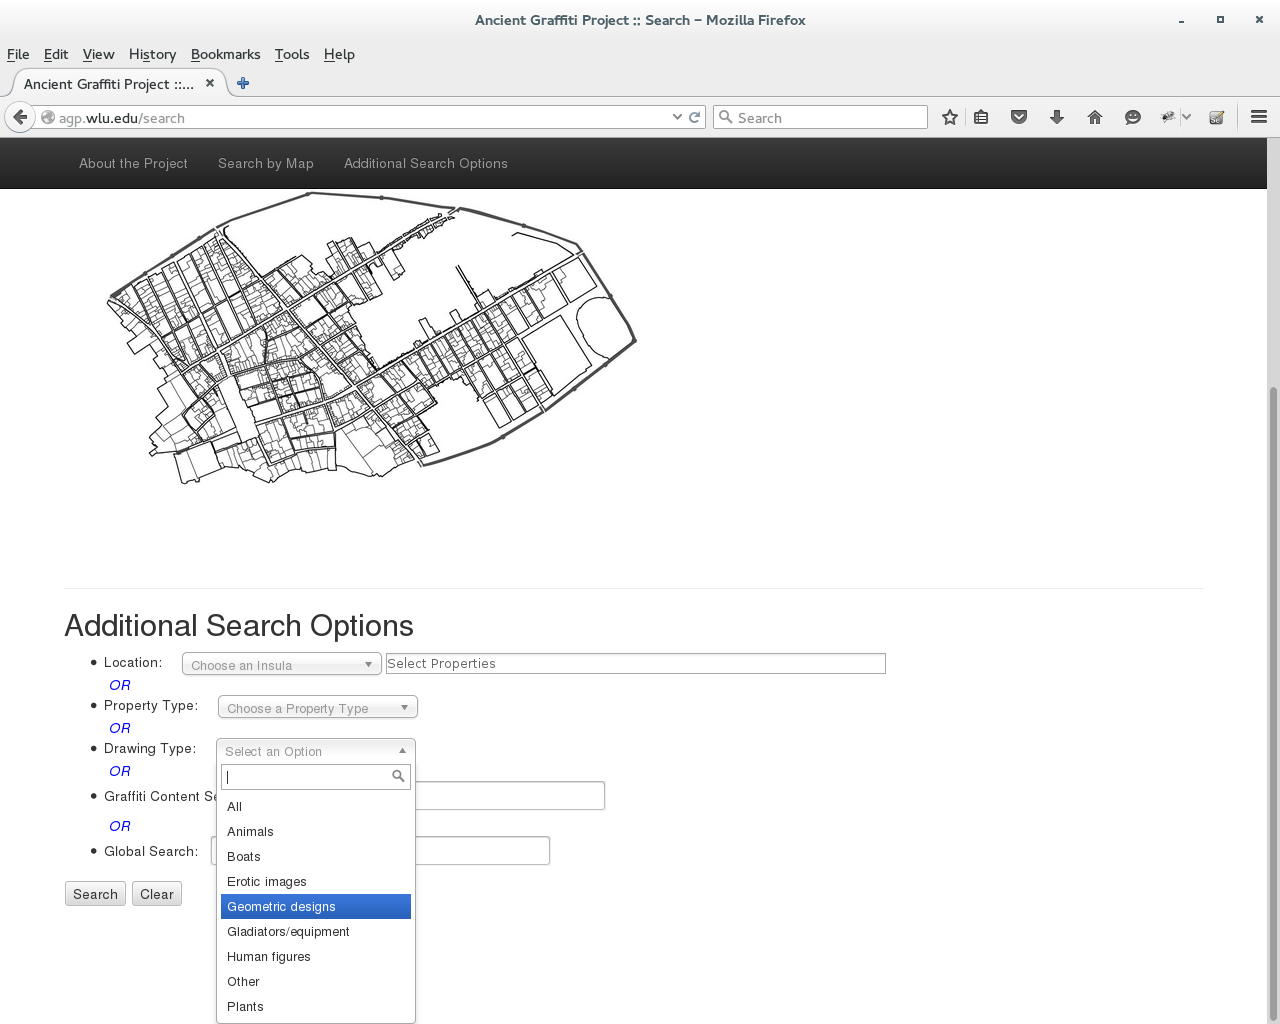
\includegraphics[width=0.9\columnwidth]{EAGLE2016BenefielSypniewski-img008.png}
\caption{Screenshot of AGP search engine showing browsing capabilities.}
\label{fig:8}
\end{figure}
 


At this point, one can browse by choosing a category, which will return all examples in that category. So, for example,
the category of ``Gladiators/equipment'' will return sketches of individual gladiators, gladiators fighting in pairs, and
gladiator equipment such as helmets. The category of ``Animals'' will return all figural graffiti that include drawings
of animals. As we process greater numbers of figural graffiti, the results of these categories will become larger.


\subsection{Limiting search results in AGP}
\noindent It is therefore necessary to design a way to limit results, so that a user could find only gladiatorial equipment,
or graffiti depicting only boars but not graffiti depicting other animals. We are developing a method of filters and
tags that will allow a user to move beyond browsing. These filters will allow a user 1) to limit an initial return of
results, 2) to retrieve more specific results, or 3) to perform a secondary level of search. It will certainly be
helpful to refine results of an entire category to include only a subset of that category, for example, only pairs of
gladiators instead of all gladiators and their equipment.

To allow for this, we are creating a list of tags that we can apply to figural graffiti to allow for greater specificity
of searching. By using tags, we can also assign multiple terms to a single image, e.g. stag and dog. Our goal is
ultimately to enable searches by these tags as well, so a user can directly find all drawings with dogs. The search
capacity will allow a user to search the tags or the Latin description, so both ``\emph{navis}'' and ``boat'' will return hits.
Again, standardization is necessary. We are currently developing a list of tags that is comprehensive and flexible
enough to cover all graffiti, but that includes a level of standardization so that the list of tags offers extensible
terms. We are also creating a system of filters to allow a user to limit the initial results or to move directly to a
desired graffito. So, a user can search all graffiti drawings and then limit the search results, for example, to find
all the drawings in a particular property [Fig.~\ref{fig:9}].


\begin{figure}[!hbp]
\centering
 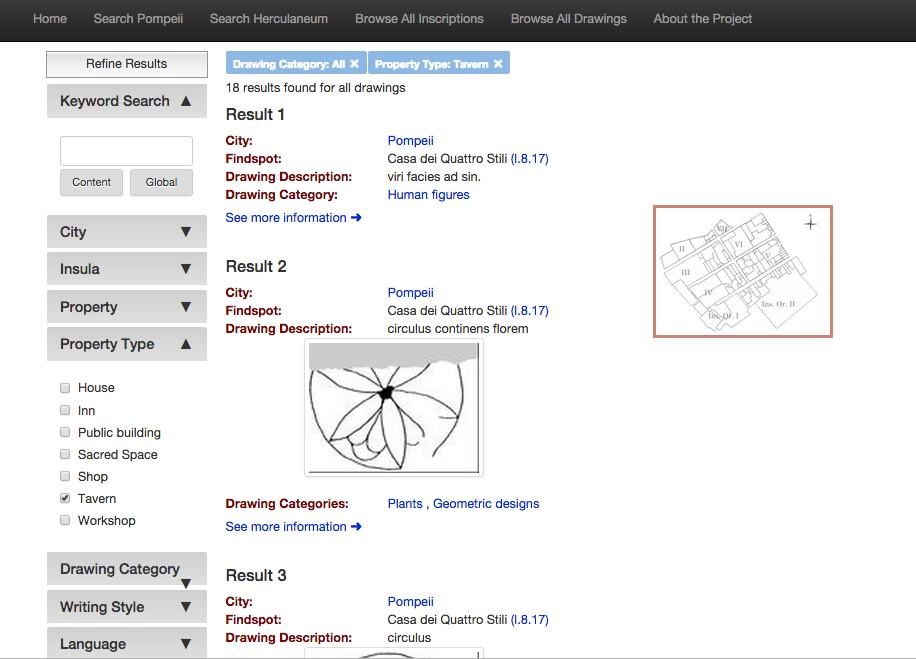
\includegraphics[width=0.9\columnwidth]{EAGLE2016BenefielSypniewski-img009.png}
\caption{Screenshot showing filters in AGP.}
\label{fig:9}
\end{figure}


Or, it will be possible to do a broad search for all drawings of animals, and then filter to limit the results to find
what kind of animals are drawn in taverns, for example, but not public buildings or houses. 




\section{Conclusion}


\noindent  This system of tags and filters is in the early stages of the design process. These are our proposed solutions for
confronting the challenges of working with text and image, and our ideas for creating a resource to complement the
strengths of EDR with search capabilities for characteristics that are specific to these heterogeneous, individualized
handwritten inscriptions. 

\nocite{wallace-hadrill_herculaneum:_2011}
\nocite{vivolo_pompei:_1993}
\nocite{guadagno_supplemento_1978}
\nocite{guadagno_supplemento_1981}
\nocite{della_corte_iscrizioni_1958}

\bibliographystyle{sapauth-eng}
\bibliography{../../EAGLE}

\end{document}